%--------------------------
\subsection{Component}
%--------------------------

Internally, a \mad component is comprised of a set of \emph{places}
linked by \emph{transitions}. The outside interface of components is
provided by their \emph{ports}, which can be bound to the internal
elements.

\paragraph{Places}{

A component in \mad is first defined by a set of places, denoted
$\Pi$. In order to define transitions and handle their
synchronization, we also introduce the notion of \emph{docks}, each
dock being attached to one place. The docks are divided between
\emph{input} and \emph{output} docks. The set of input (respectively
output) docks is denoted $\Delta_i$ (respectively $\Delta_o$), and we
use the notations $\Delta_i (\pi)$ and $\Delta_o (\pi)$ to denote the
set of input and output docks attached to a given place
$\pi$. Conversely, we denote by $\pi(d)$ the single place to which an
input or output dock $d$ is attached. A place $\pi$ such that
$\Delta_i(\pi) = \emptyset$ is said to be \emph{initial}, while if
$\Delta_o(\pi) = \emptyset$, the place is called \emph{final}.
%%Places can be part of one or multiple groups which are subsets of
%%$\Pi$. The set of groups is denoted $G$.

The set of transitions of a component is denoted
$\Theta$. A transition $\theta \in \Theta$ is a triple
$\left(s, \alpha, d\right)$ with $s\in\Delta_{o}$ an output dock,
$d\in\Delta_{i}$ an input dock, and $\alpha \in \actions$ the action
associated to the transition, taken from the set of actions $\actions$.
}

\begin{table}[tp]
  \centering
  \resizebox{\columnwidth}{!}{%
    \begin{tabular}{|c|c|}
      \hline
      & \emph{Places}\\
      \hline
      $\Pi$ & set of places of a component\\
      $\Delta_{i}$ & set of input docks of a component\\
      $\Delta_{o}$ & set of output docks of a component\\
      %$G$ & set of groups of places\\
      %$I$ & subset of places holding a token at initialization\\
      \hline
      \hline
      & \emph{Transitions}\\
      \hline
      $\Theta$ & set of transitions\\
      $\actions$ & set of actions\\
      \hline
      \hline
      & \emph{Ports}\\
      \hline
      $S_u$ & set of use ports of a component\\
      $S_p$ & set of provide ports\\
      $\types$ & set of types of ports\\
      %$type_{p}$ & function mapping a port to its type\\
      %$D_{u}$ & set of data use ports of a component\\
      %$D_{p}$ & set of data provide ports\\
      %$T_{data}$ & set of types of data ports\\
      %$type_{d}$ & function mapping a data port to its type\\
      %$\mathbb{D}$ & set of possible data values\\
      \hline
      \hline
      & \emph{Bindings}\\
      \hline
      $B_{S_{u}}$ & binding relation between use ports and transitions\\
      $B_{S_{p}}$ & binding relation between provide ports and set of places\\
      %$B_{D_{u}}$ & set of pairs mapping data use ports to transitions\\
      %$B_{D_{p}}$ & set of pairs mapping data provide ports to places\\
      \hline
      \hline
      & \emph{Assembly}\\
      \hline
      $C$ & set of components of an assembly\\
      $L$ & set of use-provide connections of an assembly\\
      %$L_D$ & set of data-use-provide connections of an assembly\\
      \hline
      \hline
      & \emph{Semantics}\\
      \hline
      $\mk$ & subset of elements holding a token\\
      $\reached$ & subset of places that have been reached\\
      $\exec$ & set of ongoing actions\\
      \hline
    \end{tabular}
  }
  \caption{Defining element of the \mad formal model}
  \label{tab:not}
\end{table}

\paragraph{Ports and bindings}{

The ports of a component are divided between a set of \emph{provide
  ports} denoted $S_p$ and a set of \emph{use ports} denoted
$S_u$. Ports are given a type among a set of types $\types$. The type
of a given port $p$ is denoted $\types(p)$. This simple typing
discipline is a way to distinguish categories of services or data that
ports may provide or use.

A provide port may be bound to sets of place. A provide port becomes
\emph{enabled} if all the sets of places to which it is bound include
at least one place that has been reached. This binding relation is
denoted $B_{S_p} \subseteq S_p \times \mathcal{P}(G)$. Intuitively,
bindings allow the modeling of conjunctions (all sets of places must
be reached) and disjunctions (one set of place is reached if at least
one of its place is reached) of constraints to control the enabling of
provide ports. Note that once a port is enabled, it remains in that
state forever.

A use port may be bound to transitions, indicating that those
transitions can be fired only if the port is \emph{provided}, \ie
connected to an enabled provide port. This binding relation is denoted
$B_{S_{u}} \subseteq S_u \times \Theta$.

%% SR remove the distinctinction between data and "regular" ports, all 

%% In addition to traditional use-provide ports of component models,
%% \mad handles a specific use-provide abstraction for the
%% transfer of data values. These ports are called \emph{data-use-ports}
%% and \emph{data-provide-ports}. The set of data-use ports is denoted
%% $D_{u}$, and the set of data-provide ports is denoted
%% $D_{p}$. Each data port is associated to a type in $T_{data}$,
%% and the set of possible data values is denoted
%% by $\mathbb{D}$. Finally, the function $type_{d}\,:\,D_{u}\cup
%% D_{p}\rightarrow T_{data}$ maps data ports to their data type.

%% A port can be bound to places, groups of places or transitions.
%% There are four types of bindings.  First, we
%% denote by $B_{S_{u}} \subseteq S_u \times \Theta$ the binding
%% relation between use ports and transitions of the component. A
%% transition can be fired only if its bound ports are enabled. Second,
%% we denote by $B_{S_{p}} \subseteq S_p \times \mathcal{P}(G)$ the binding relation
%% between provide ports and groups of places. A provide port is
%% enabled only when all the group to which it is bound hold at least
%% one token. Third, we denote by $B_{D_{u}} \subseteq D_u \times
%% \Theta$ the binding relation between data use ports and transitions
%% of the component, indicating that transition uses the data
%% associated with the bound ports. Finally, we denote by $B_{D_{p}}
%% \subseteq D_p \times \pi$ the binding relation between data provide
%% ports and places place, indicating that the data associated to a
%% port is available only if the places to which it is bound hold (or
%% have held) a token. Note that there is no restriction on the number
%% of bindings for each port.
}

%--------------------------
\subsection{Assembly}
%--------------------------

An \emph{assembly} of components represents the instantiation of
components as defined in the previous section, and their connections
through their ports. In \mad, an assembly is defined as a pair $(C,
L)$, where $C$ is a set of components, and $L \subseteq S_u^*
\times S_p^*$ is the set of connections (links) between use ports and
provide ports. For all the components $c_1,\dots,c_n \in C$, we denote
with a star any union of the corresponding sets, for instance
$\Pi^*=\bigcup_{i=1}^{n}\Pi_{i}$. Linked ports must be of compatible
types, \ie $(u,p) \in L$ only if $\types(u) = \types(p)$.

%--------------------------
\subsection{Operational semantics}
\label{subsec:operational_semantics}
%--------------------------

At each moment in the execution of a \mad deployment assembly
$(C, L)$, the \emph{configuration} of this assembly is defined by a
tuple $\langle \mk, \reached, \exec \rangle$, where

\begin{itemize}
  \item $\mk \subseteq \Pi^{*} \cup
    \Delta_{i}^{*}\cup\Delta_{o}^{*}\cup\Theta^{*}$ denotes the
    elements that hold a token;
  \item $\reached \subseteq \Pi^*$ denotes the places that have been
    reached;
  \item $\exec \subseteq A$ denotes the actions that are being executed.
\end{itemize}

The initial configuration of an assembly is given by $\langle I, I,
\emptyset\rangle$, where $I = \{ \pi \, \mid \, \Delta_i(\pi) =
\emptyset \}$ (\ie the set of initial places).

%% \noindent\textbf{Terminology.}

%% \begin{figure}[t]
%%   \begin{center}
%%     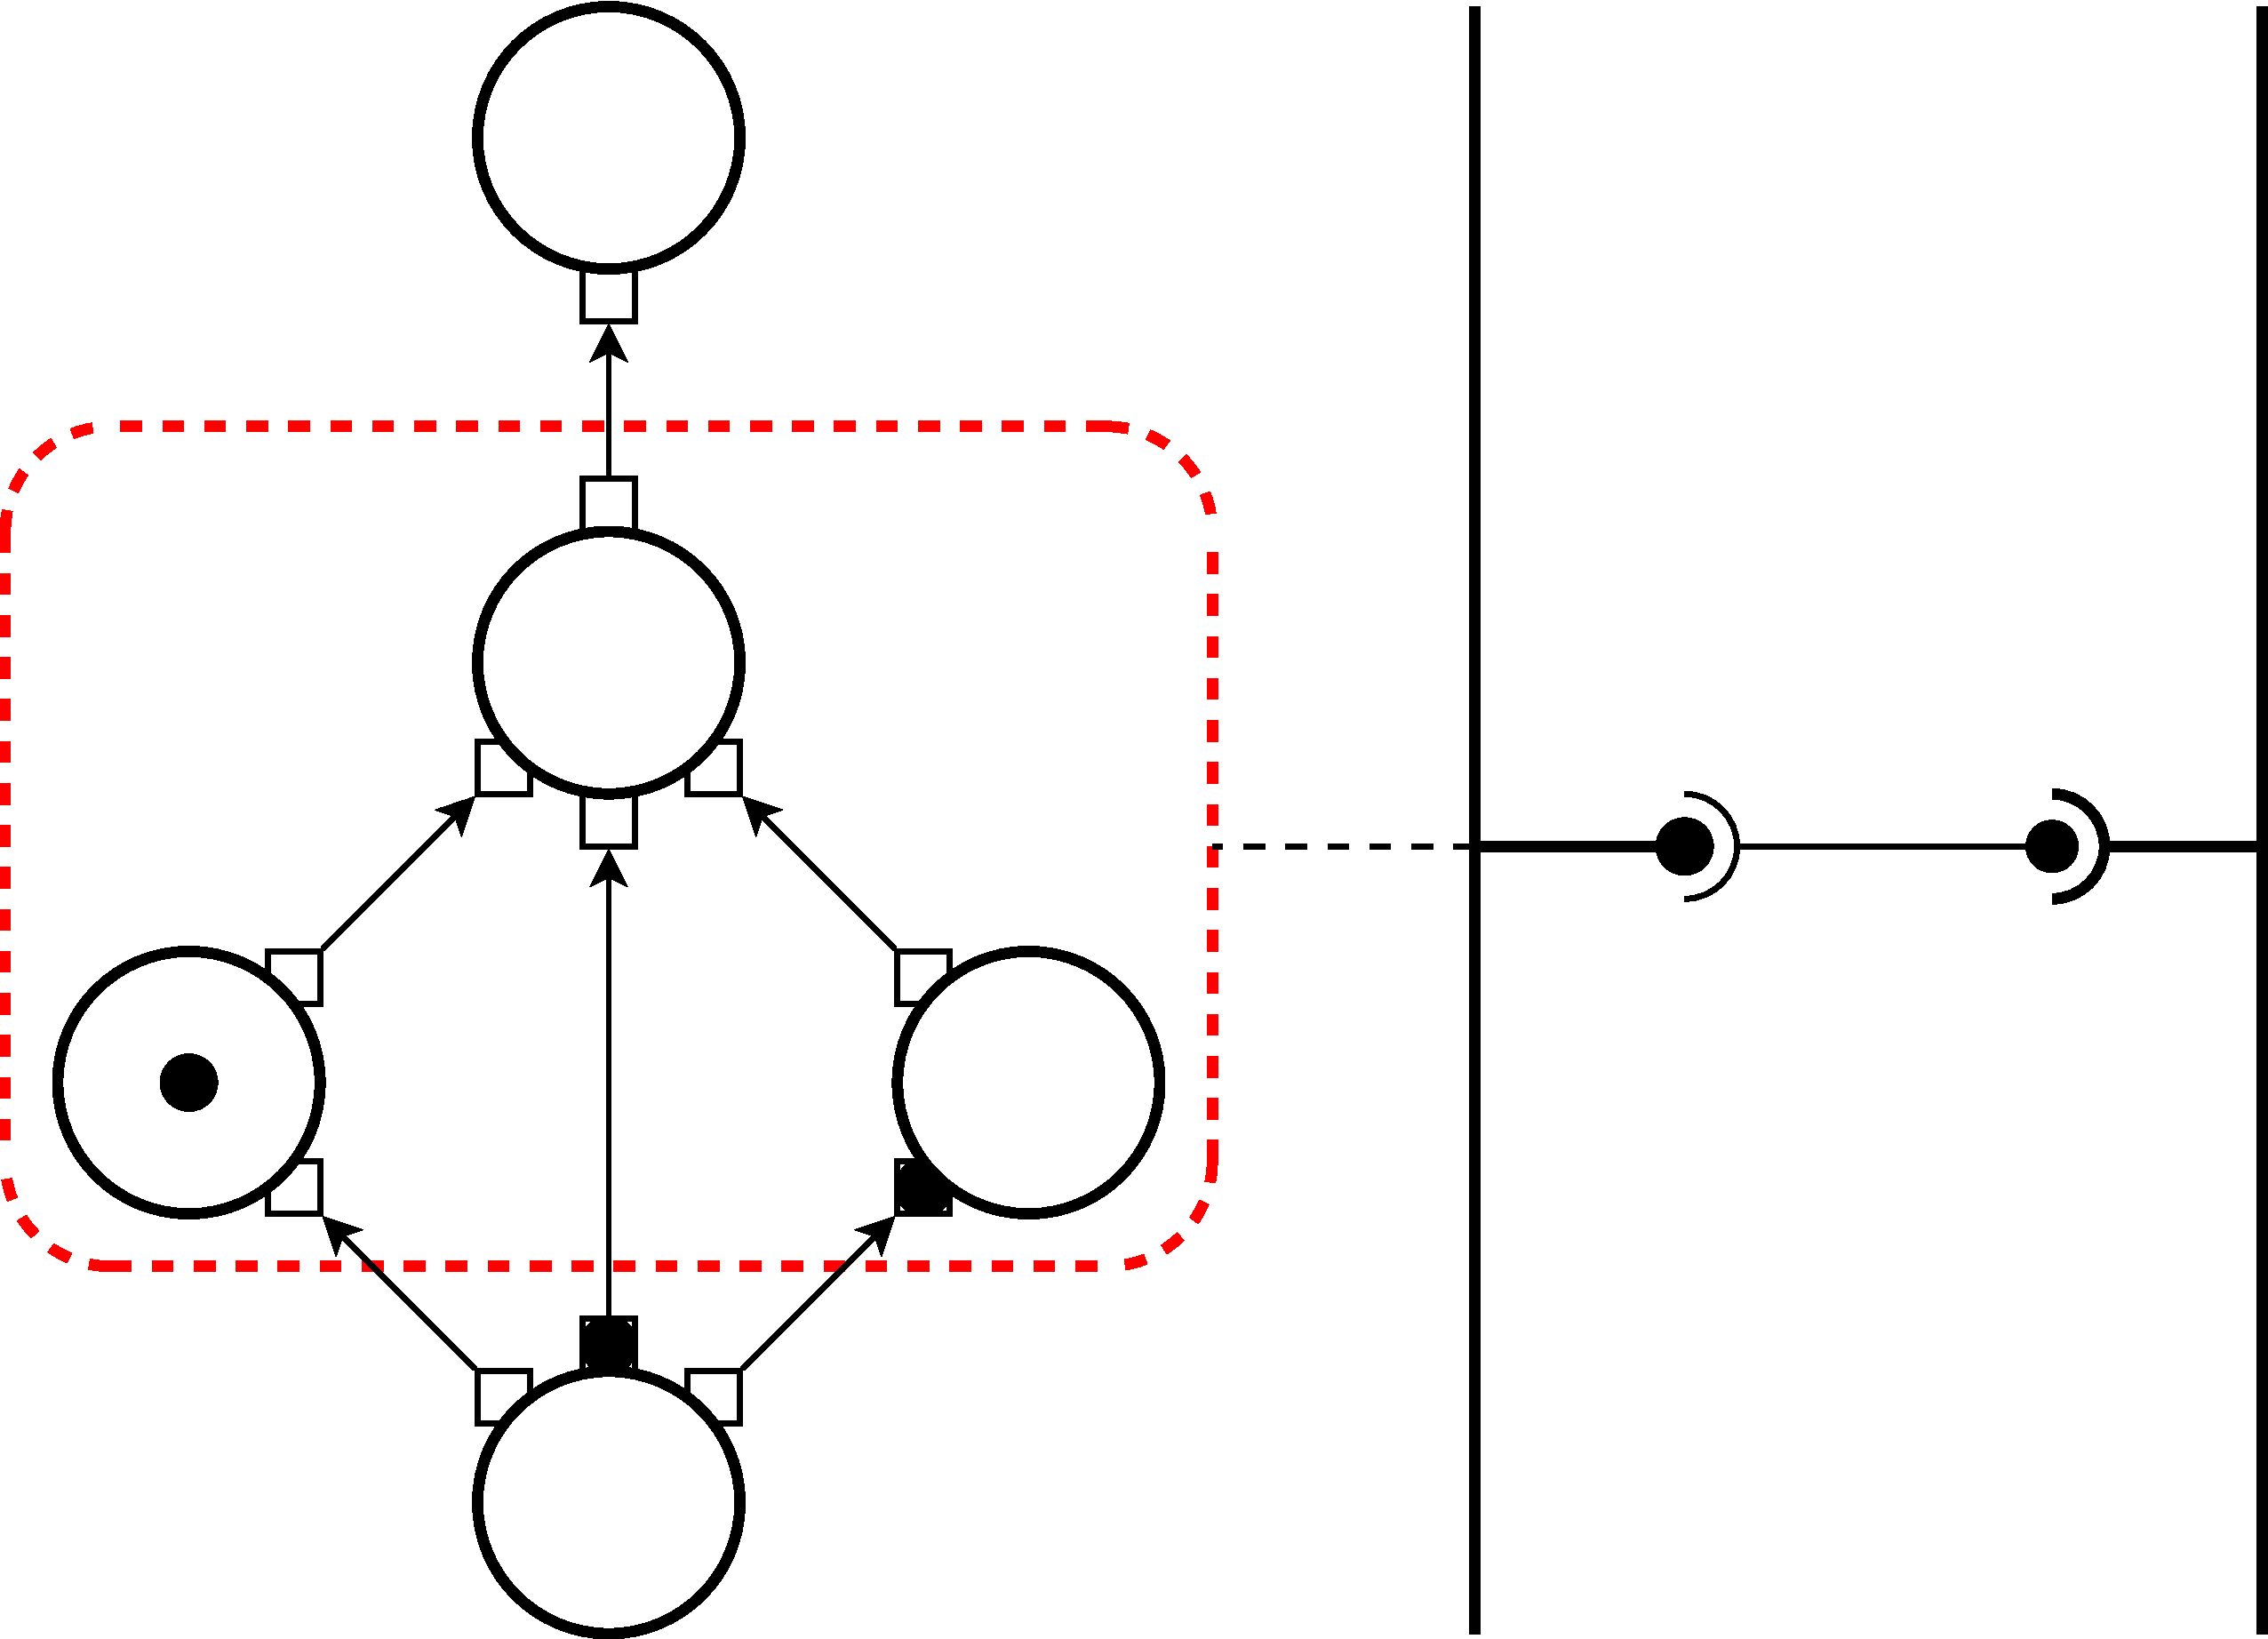
\includegraphics[width=0.7\columnwidth]{./images/enabled_service.pdf}

%%     \caption{The connection is enabled because its provide port is enabled, as all the groups it is bound to hold a token.}

%%     \label{fig:enabled_service}
%%   \end{center}
%% \end{figure}

%% \begin{figure}[t]
%% \begin{center}
%%   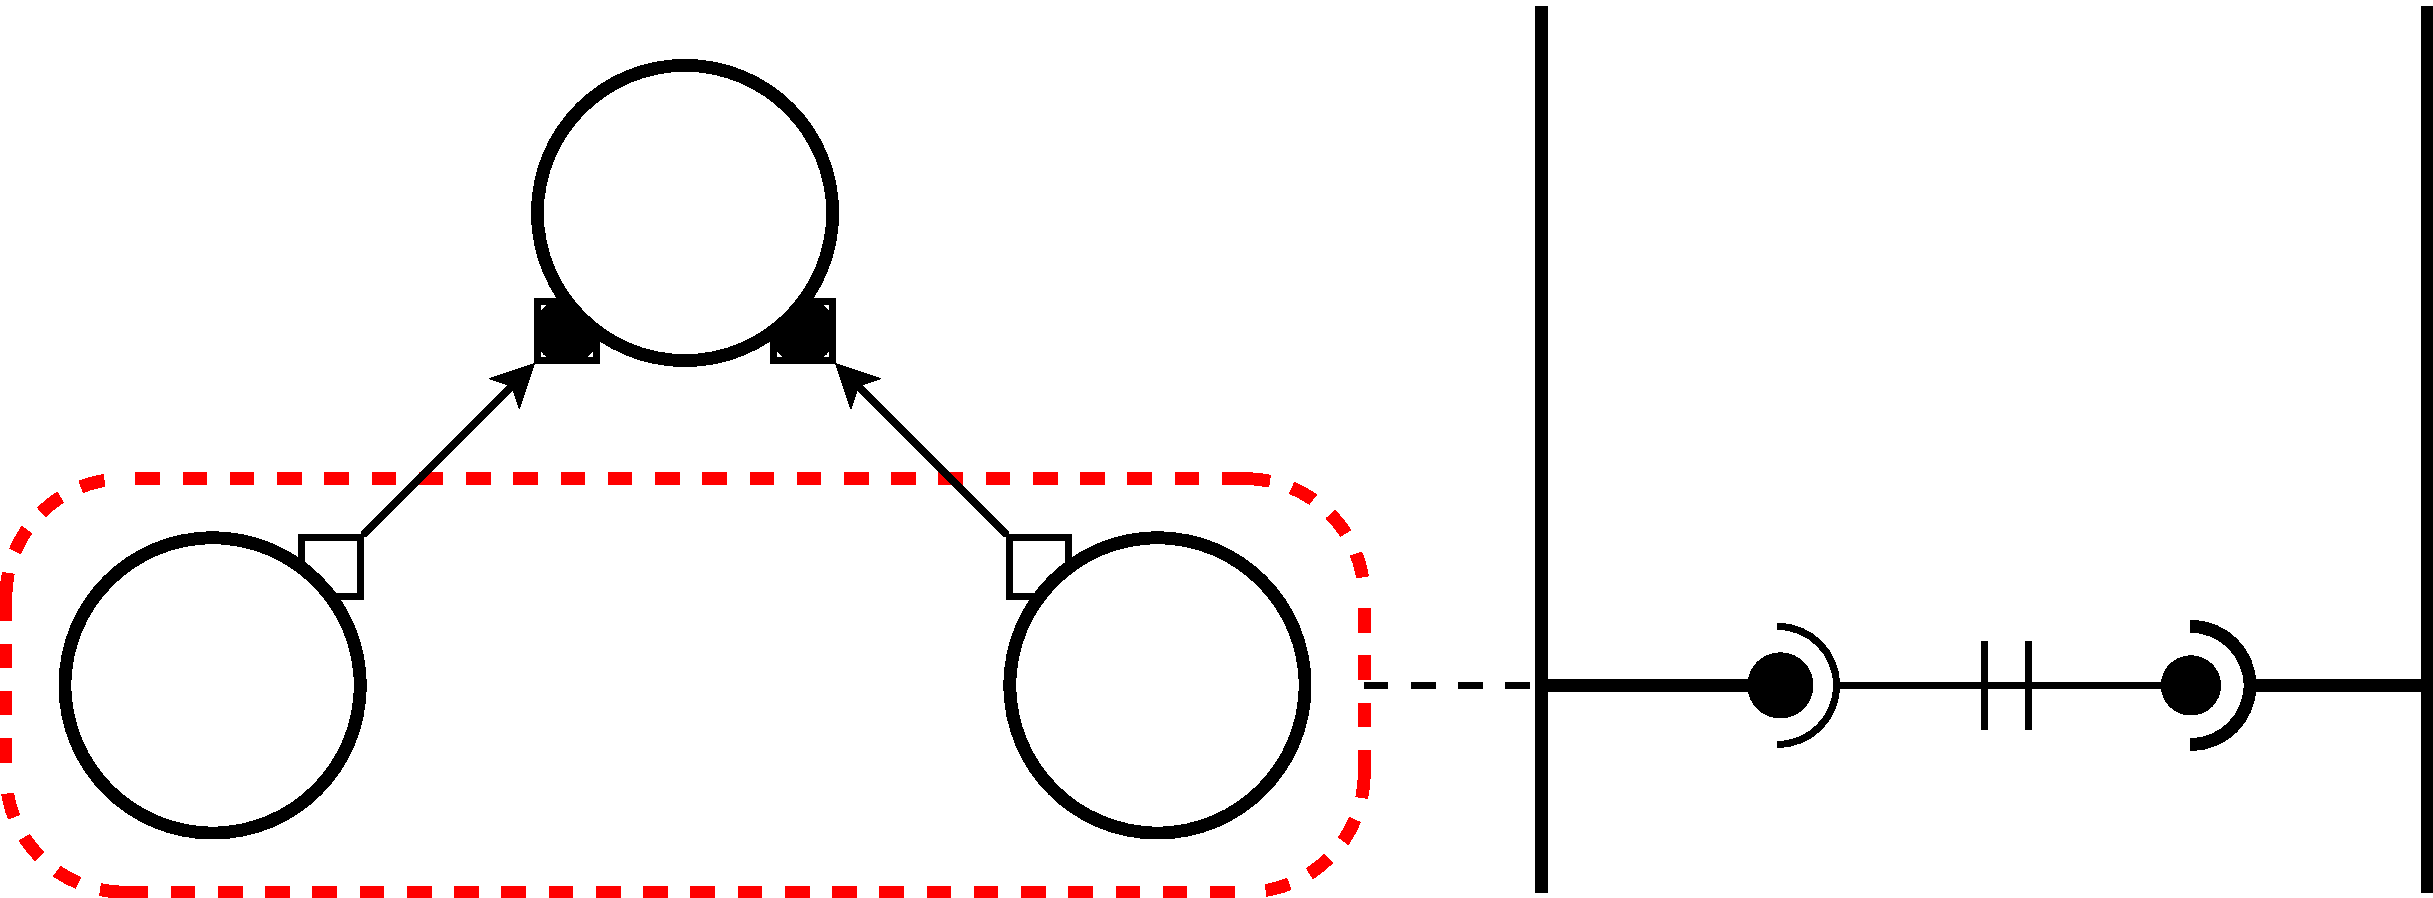
\includegraphics[width=0.7\columnwidth]{./images/disabled_service.pdf}
%% \end{center}
%% \caption{The connection is disabled because its provide port is disabled, as one of the groups it is bound to does not hold a token.}
%% \label{fig:disabled_service}
%% \end{figure}

%% \begin{figure}[t]
%% \begin{center}
%%   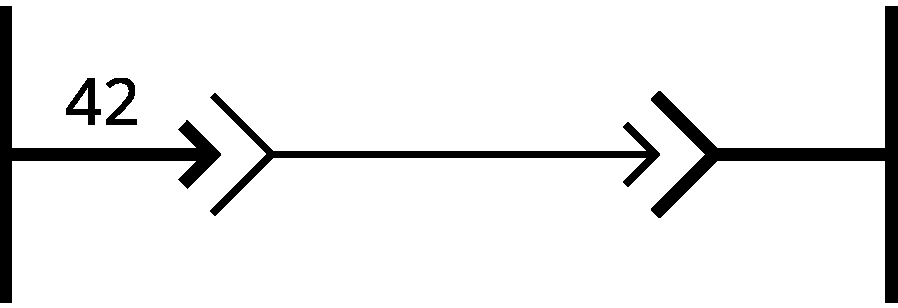
\includegraphics[width=0.4\columnwidth]{./images/enabled_data.pdf}
%% \end{center}
%% \caption{The connection is enabled because its data-provide port holds a value.}
%% \label{fig:enabled_data}
%% \end{figure}

%% \begin{figure}[t]
%% \begin{center}
%%   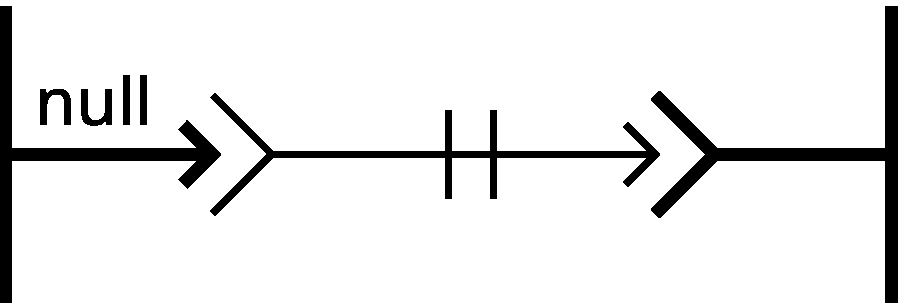
\includegraphics[width=0.4\columnwidth]{./images/disabled_data.pdf}
%% \end{center}
%% \caption{The connection is disabled because its data-provide port does not hold a value.}
%% \label{fig:disabled_data}
%% \end{figure}

%% A group is enabled if it contains at least one token, and a
%% service-provide port is enabled if all the groups it is bound to are
%% enabled. A service connection is enabled if its provide port is
%% enabled. A group, port, or connection that is not enabled is said to
%% be disabled. Figure~\ref{fig:enabled_service} gives an example of an
%% enabled service connection, while Figure~\ref{fig:disabled_service}
%% gives an example of a disabled service connection.

%% A data-provide port is enabled if it holds a value, and a data
%% connection is enabled if its provide port is enabled disabled).
%% Figure~\ref{fig:enabled_data} gives an example of an enabled data
%% connection, while Figure~\ref{fig:disabled_data} gives an example of a
%% disabled data connection.
    
We now formally present the operational semantics of the \mad model,
given as a binary relation $\semstep$ over configurations. The rules
describing this relation are given in Figure \ref{fig:rules}.

An execution of an assembly $A$ is a sequence of configurations
\[
\langle I, I, \emptyset \rangle \semstep \langle \mk_1, \reached_1, \exec_1 \rangle \semstep \semstep \langle \mk_2, \reached_2, \exec_2 \rangle \semstep \dots
\]
An execution may be finite only if the last configuration $\langle
\mk_n, \reached_n, \exec_n \rangle$ is such that no rule applies.

\paragraph{Reaching place}{

The rule $\reachplace$ describes the activation of a place $\pi$. It
requires that all the input docks connected to the place hold a
token. In the conclusion, those tokens are removed from the docks, and
one token is placed on $\pi$, as illustrated in Figure~\ref{fig:r3}.

\begin{figure}[t]

\begin{minipage}[h]{0.45\columnwidth}%
  \centering
  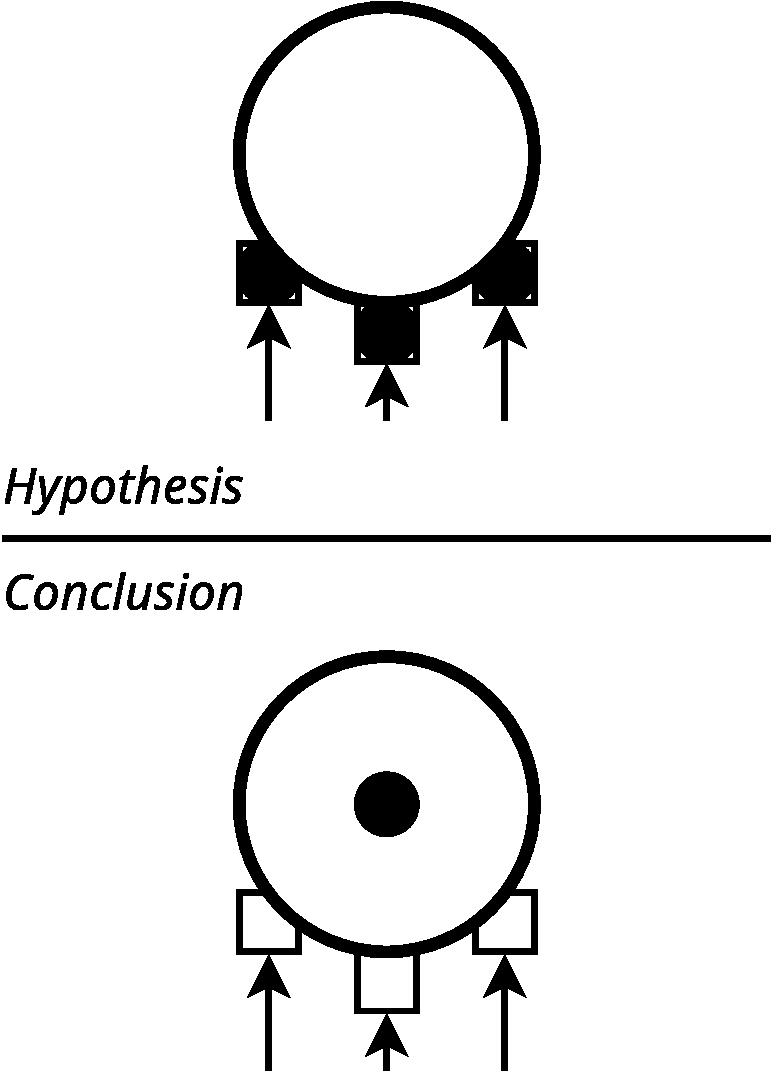
\includegraphics[width=0.65\columnwidth]{./images/inputdocks_to_place.pdf}
  \captionof{figure}{\label{fig:r3}Illustration of the rule of $\reachplace$.}
\end{minipage}
\hfill
\begin{minipage}[h]{0.45\columnwidth}%
  \centering
  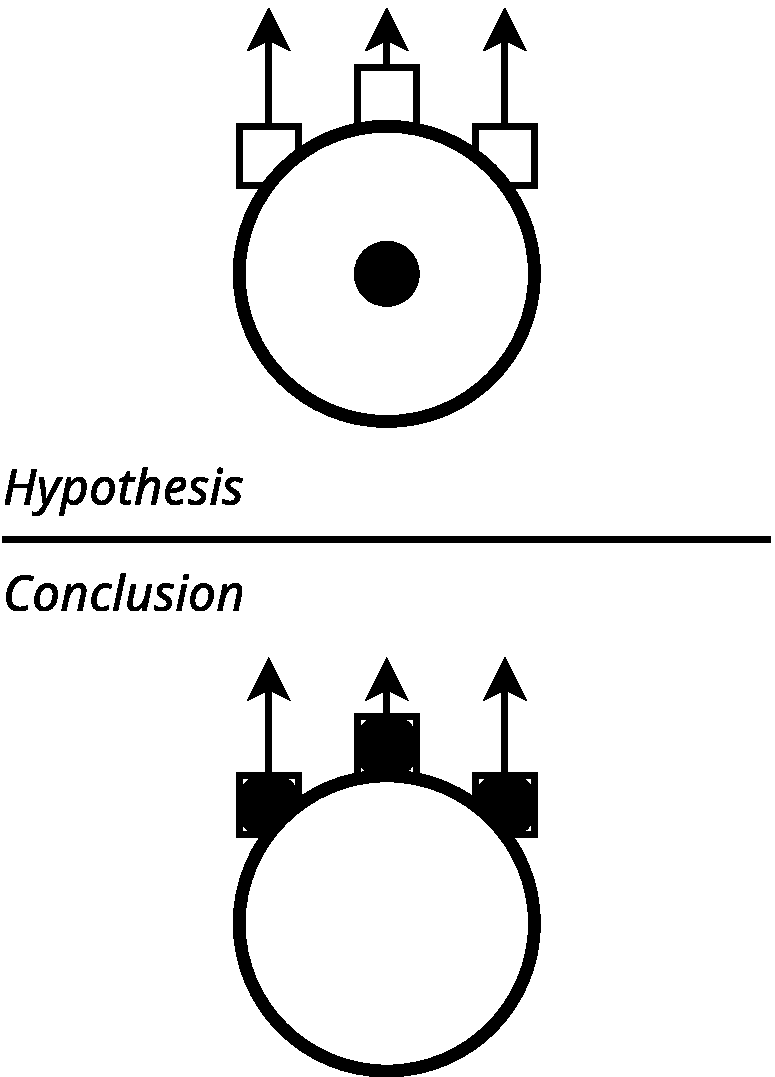
\includegraphics[width=0.65\columnwidth]{./images/place_to_outputdocks.pdf}
  \captionof{figure}{\label{fig:r4}Illustration of the rule $\leaveplace$.}
\end{minipage}
\end{figure}

\paragraph{Leaving place}{
  
The rule $\leaveplace$ defines the transfer of a token from a place
$\pi$. The token is be removed from $\pi$, and a token added to each
output dock attached to $\pi$. This rule is illustrated in
Figure~\ref{fig:r4}.

}

\paragraph{Firing transition}{

The rule $\firetrans$ corresponds to the firing of a transition
$\theta = (s, \alpha, d)$. The output dock $s$ must hold a token, and
any use port bound to $\theta$ must be provided. The token is
transfered from the input dock to the transition itself, and the
action $\alpha$ is executed, as illustrated in Figure~\ref{fig:r1}

\begin{figure}[t]
\begin{center}
  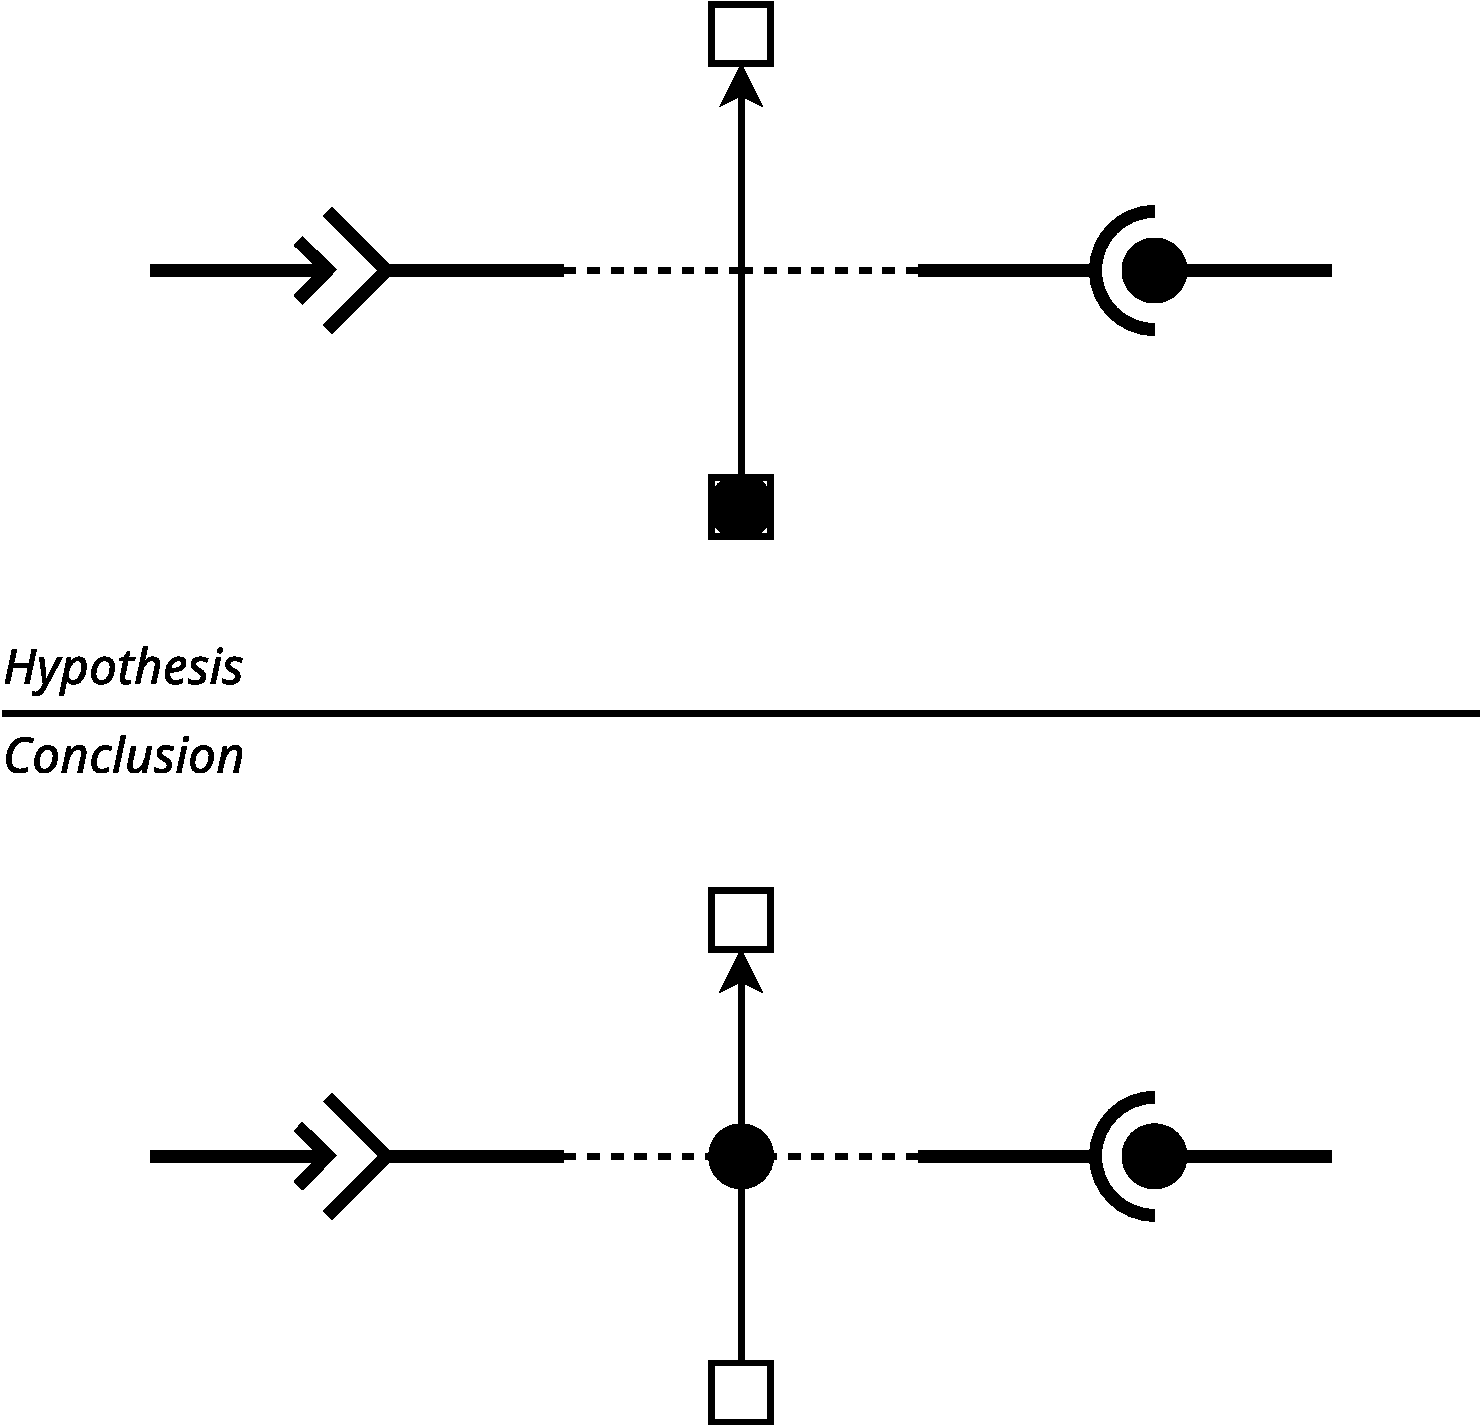
\includegraphics[width=0.55\columnwidth]{./images/firing.pdf}
\end{center}
\caption{Illustration of the rule $\firetrans$.}
\label{fig:r1}
\end{figure}

}

\paragraph{Terminating action}{
  The rule $\terminaction$ corresponds to the termination of an action
  $\alpha$. Any such action in $\exec$ can be removed by this rule.
}

\paragraph{Ending transition}{

The rule $\leavetrans$ formally describes the end of a transition
$\theta = (s, \alpha, d)$. It requires that $\theta$ holds a token and
that the action $\alpha$ has terminated. When ending a transition, the
token is moved from $\theta$ to the input dock
$d$. Figure~\ref{fig:r2} illustrates this rule.

\begin{figure}[t]
\begin{center}
  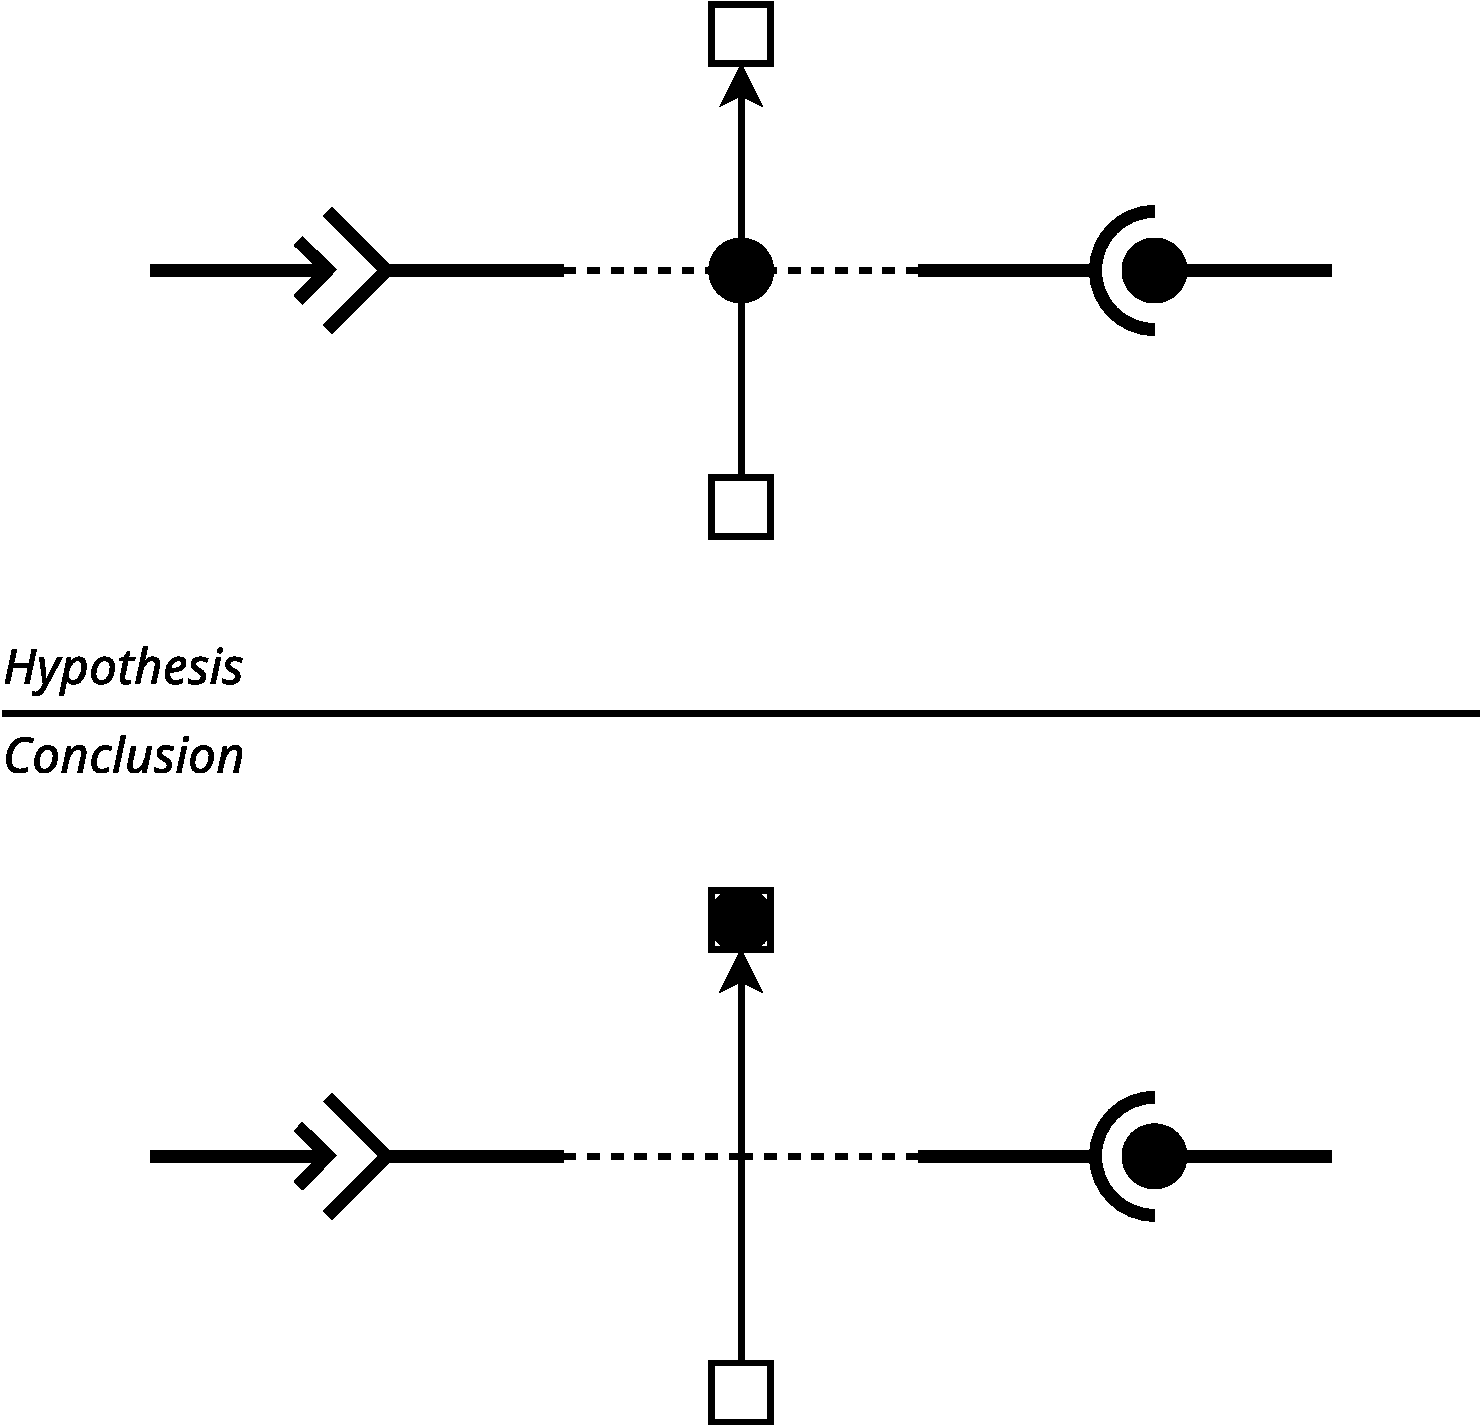
\includegraphics[width=0.55\columnwidth]{./images/ending_transition.pdf}
\end{center}
\caption{Illustration of the rule $\leavetrans$.}
\label{fig:r2}
\end{figure}
  
}

%% \MC{Pour moi il faut séparer la fin des actions et des transitions et
%% ajouter une règle ``l'action se termine'' avec précondition ``l'action est en cours''}
%% SR : fait

%------------
\begin{figure*}[tp]
  \begin{prooftree}
    \AxiomC{$\pi\in\Pi^*$}
    \AxiomC{$\emptyset \subset \Delta_i(\pi) \subseteq  \mk$}
    \RightLabel{$\reachplace$}
    \BinaryInfC{$\langle \mk, \reached, \exec \rangle \semstep \langle (\mk \setminus \Delta_i(\pi)) \cup \{ \pi \}, \reached \cup \{ \pi \} , \exec\rangle$}
  \end{prooftree}
  
  \begin{prooftree}
    \AxiomC{$\pi\in\Pi^{*}$}
    \AxiomC{$\pi \in \mk$}
    %\AxiomC{$\forall g\in G, \pi\in g:\,\text{can\_leave}(\pi, \Delta_o(\pi) ,g)$}
    \RightLabel{$\leaveplace$}
    \BinaryInfC{$\langle \mk, \reached, \exec \rangle \semstep \langle (\mk \setminus \{ \pi \}) \cup \Delta_o(\pi), \reached, \exec\rangle$}
  \end{prooftree}
  %
  \begin{prooftree}
    \AxiomC{$\theta = \left(s,\alpha,d\right) \in \Theta^*$}
    \AxiomC{$s \in \mk$}
    \AxiomC{$\forall p. \; (p,\theta) \in B_{S_u}^* \implies provided(p)$}
    \RightLabel{$\firetrans$}
    \TrinaryInfC{$\langle \mk, \reached, \exec \rangle \semstep \langle (\mk \setminus \{ s \}) \cup \{\theta\}, \reached, \exec \cup \{ \alpha \}\rangle$}
  \end{prooftree}
  %
  where
  \[
  provided(p) \equiv \exists u. \; (u,p) \in L \land (\forall G. \; (p, G) \in B_{S_p}^* \implies G \cap \reached \neq \emptyset)
  \]
  %% \begin{align*}
  %%   \text{where: }provided(p) \equiv &\, \exists u \, (u,p) \in L \land enabled_c\left((u,p)\right) \\
  %%   enabled_c\left((u,p)\right) \equiv &\, \forall g\in G,\left(p,g\right)\in B_{S_{p}}\,:\,enabled_g\left(g,\mk\right) & \text{if }\left(u,p\right)\in L\\
  %%   enabled_g\left(g,\mk\right) \equiv & \left(\exists\,\pi\in g : \pi \in \mk\right)\\
  %%   & \, \lor\left(\exists \theta = (s,\alpha,d)\in\Theta^{*}:\,\left(\theta \in \mk \lor s \in \mk \lor d \in \mk\right)\land \pi(s)\in g \land \pi(d)\in g\right)
  %% \end{align*}

  \begin{prooftree}
    \AxiomC{$\alpha \in \exec$}
    \RightLabel{$\terminaction$}
    \UnaryInfC{$\langle \mk, \reached, \exec \rangle \semstep \langle \mk, \reached, \exec \setminus \{ \alpha \} \rangle$}
  \end{prooftree}
  
  \begin{prooftree}
    \AxiomC{$\theta=\left(s,\alpha,d\right) \in \Theta^*$}
    \AxiomC{$\theta \in \mk$}
    \AxiomC{$\alpha \not\in \exec$}
    \RightLabel{$\leavetrans$}
    \TrinaryInfC{$\langle \mk, \reached, \exec \rangle \semstep \langle ((\mk \setminus \{ \theta \}) \cup \{ d \}, \reached ,\exec \rangle$}
  \end{prooftree}
  
  %
  %% \begin{align*}
  %%   \text{where: }\text{can\_leave}\left(\pi,D_o,g\right) = & \left(\exists p,(p,g)\in B_{S_p}:\,locked(p)\right)\implies \lnot \text{last\_token\_leaves} \left(\pi,D_o,g\right) \\
  %%   locked\left(p\right) = & \exists u\in S_{u}^{*},\theta\in\Theta^{*}:~\left(p,u\right)\in L_S\land \left(u,\theta\right)\in B_{S_u}^{*}\land \theta \in \mk \\
  %%   \text{last\_token\_leaves}\left(\pi,D_o,g\right) = & \left(\text{is\_group\_enabled}\left(g,\mk\right)\land\lnot \text{is\_group\_enabled} \left(g,(\mk \setminus \{ \pi \}) \cup D_o\right)\right) \\
  %% \end{align*}
  %
  \caption{The operational semantics of \mad.}
  \label{fig:rules}
\end{figure*}
%------------

%--------------------------
%\subsection{Consistency rule}
%--------------------------

\paragraph{Structural constraints}{
  A place $\pi_1$ is said to \emph{precede} a place $\pi_2$ if there
  exists $(s, \alpha, d) \in \Theta$ such that $\pi(s) = \pi_1$ and
  $\pi(d) = \pi_2$.  If there exists a sequence $(\pi_1, \pi_2, \dots,
  \pi_n)$, such that $\pi_{i}$ precedes $\pi_{i+1}$ for any $i$ where
  $1 \le i < n$, then we say that $\pi_n$ \emph{depends} on $\pi_1$.

  A \mad component is said to be \emph{well-formed} if there exists no
  place $\pi$ that depends on itself. Intuitively, the component,
  viewed as a directed graph, must be acyclic.

  The lemmas below all assume an assembly $A = (C, L)$ such that all
  components $c \in C$ are well-formed.

  \begin{lemma}\label{thm:finite}
    Any execution of $A$ is finite.
  \end{lemma}

  \begin{proof}
    By contradiction, assume that there exists an infinite execution
    of $A$. Since the sets of places, docks, transitions and actions
    are finite, the set of configurations is also finite. Therefore
    the execution must reach the same configuration more than once,
    \ie it has a prefix
    \[
    \langle I, I, \emptyset \rangle \semstep \dots \semstep \langle \mk, \reached, \exec \rangle_i \semstep \dots \semstep \langle \mk, \reached, \exec \rangle_j
    \]
    such that $\langle \mk, \reached, \exec \rangle_i = \langle \mk,
    \reached, \exec \rangle_j$.

    Let us denote $\reached^+$ the set of places that are reached more
    than once. By case analysis over the relation $\langle \mk,
    \reached, \exec \rangle_i \semstep \langle \mk, \reached, \exec
    \rangle_{i+1}$, we can check that $\reached^+$ is non-empty.
    \begin{itemize}
    \item for the case of the rule $\leaveplace$, a token is removed
      from the place $\pi$, therefore a token must be placed back on
      $\pi$ to attain configuration $\langle \mk, \reached, \exec
      \rangle_j$ ;
    \item for the case of the rules $\reachplace$, $\firetrans$,
      $\terminaction$ and $\leavetrans$, there must exist a transition
      $\theta = (s, \alpha, d)$ such that $\pi(s)$ is reached
      more than once.
    \end{itemize}
    Furthermore, because all components are well-formed, the
    precede-relation over places is well-founded, therefore there
    exists at least one place $\pi \in \reached^+$ such that all
    places $\pi'$ that precede $\pi$ are in $\Pi \setminus
    \reached^+$. This place is reached more than once, but all the
    places that precede it have been reached at most one time, leading
    to a contradiction.
  \end{proof}

  \begin{lemma}\label{thm:applyrules}
    For any execution of $A$, if the conditions of a rule are
    eventually satisfied, this rule will eventually be applied.
  \end{lemma}

  \begin{proof}
    We can see that, for any execution and any condition of a rule,
    either the condition remains true forever (in particular, reached
    places and provided ports remain in that state) or the condition
    remains true until the rule is applied (\eg a token is moved by
    the rule).

    By Lemma~\ref{thm:finite}, all executions must be finite, and by
    definition of an execution, no rule should be applicable in the
    final configuration.
  \end{proof}

  \begin{lemma}\label{thm:reachedplaces}
    Let $c \in C$ be a component, and $\pi$ a place in it. In any
    execution of $A$, if all places $\pi'$ that precede $\pi$ are
    eventually reached, and all use ports of $c$ are eventually
    provided, then $\pi$ is eventually reached.
  \end{lemma}

  \begin{proof}
    Let us consider an execution such that (i) all places $\pi'$ that
    precede $\pi$ are eventually reached, and (ii) all use ports of
    $c$ are eventually provided.

    If $\Delta_i(\pi) = \emptyset$, then $\pi \in I$ and $\pi$ is
    reached in the initial configuration.
    
    Otherwise, for each place $\pi'$ and each transition $\theta = (s,
    \alpha, d)$ where $\pi(s) = \pi'$ and $\pi(d) = \pi$, by (i),
    $\pi'$ must eventually hold a token. By
    Lemma~\ref{thm:applyrules}, $\theta$ must eventually be fired,
    $\alpha$ be terminated and $\theta$ be ended (rules $\firetrans$,
    $\terminaction$ and $\leavetrans$), thus any $d \in \Delta_i(\pi)$
    will eventually hold a token. Furthermore, tokens are removed from
    $\Delta_i(\pi)$ only when $\pi$ is reached (rule $\reachplace$),
    hence the conditions of $\reachplace$ will eventually be
    satisfied, and $\pi$ reached.
  \end{proof}
  
  \begin{lemma}
    Let $c$ be a well-formed component. For any execution where all
    use ports $u \in S_u$ are eventually provided, all places of $c$
    will eventually be reached.
  \end{lemma}

  \begin{proof}
    By contradiction, assume the existence of an execution such that
    (i) some place of $c$ is never reached and (ii) all use ports are
    eventually provided.

    Let $\reached^\omega$ denote the set of places that are eventually
    reached in that execution. By (i), the set $\Pi \setminus
    \reached^\omega$ is non-empty. Furthermore, because $c$ is
    well-formed, the precede-relation is well-founded, therefore there
    exists at least one place $\pi \in \Pi \setminus \reached^\omega$
    such that all places $\pi'$ that precede $\pi$ are in
    $\reached^\omega$. By (ii) and Lemma~\ref{thm:reachedplaces}, $\pi
    \in \reached^\omega$, leading to a contradiction.
  \end{proof}

  This lemma indicates that the \mad model provides, by construction,
  a guarantee of reachability at the component level, \ie deadlocks
  cannot occur within a component. At the level of an assembly, we
  cannot enforce similar structural constraints, because the different
  components are typically developed independently from each other,
  often by different actors. For this reason, reachability guarantees
  cannot be offered on assemblies. Instead we must rely on analysis of
  a given assembly. One way to perform this analysis is to use
  model-checking~\cite{coullon:hal-02323641}, but for most assemblies,
  a simpler analysis tool can be used.
}

\paragraph{Consistency}{

  \SR{Keep? Move somewhere else?}
  
  In \mad, the maximum number of tokens that can be used is the
  maximum number of possible parallel branches. A token can only be
  created during a branching (rule $\leaveplace$), where one token is
  created for each output dock of the place. Because components are
  well-formed, places can be reached (and therefore, left) at most
  once, so the maximum number of tokens that can be present in a
  component is bounded. We plan in future work to support
  reconfiguration to allow cycles in very specific settings to keep
  control on the tokens and their creation.
}
